\documentclass{article}
\usepackage{fullpage,booktabs,graphicx,hyperref,float,array}
% generated by grnbench report from result files - do not edit
\newcommand{\gbCiHighAuprcRatioAutoGrnboostTwoMotifVsGrnboostTwo}{+0.173}
\newcommand{\gbCiHighAuprcRatioAutoGrnboostTwoVsPearsonSigned}{-0.161}
\newcommand{\gbCiHighAuprcRatioAutoPearsonMotifVsPearsonSigned}{+0.259}
\newcommand{\gbCiHighAuprcRatioAutoRegdiffusionMotifVsRegdiffusion}{+0.296}
\newcommand{\gbCiHighAuprcRatioAutoRegdiffusionVsPearsonSigned}{+0.133}
\newcommand{\gbCiHighAuprcRatioBaselineGrnboostTwoMotifVsGrnboostTwo}{+0.167}
\newcommand{\gbCiHighAuprcRatioBaselineGrnboostTwoVsPearsonSigned}{-0.130}
\newcommand{\gbCiHighAuprcRatioBaselinePearsonMotifVsPearsonSigned}{+0.245}
\newcommand{\gbCiHighAuprcRatioBaselineRegdiffusionMotifVsRegdiffusion}{+0.278}
\newcommand{\gbCiHighAuprcRatioBaselineRegdiffusionVsPearsonSigned}{+0.144}
\newcommand{\gbCiHighEprAutoGrnboostTwoMotifVsGrnboostTwo}{+0.684}
\newcommand{\gbCiHighEprAutoGrnboostTwoVsPearsonSigned}{-0.665}
\newcommand{\gbCiHighEprAutoPearsonMotifVsPearsonSigned}{+0.303}
\newcommand{\gbCiHighEprAutoRegdiffusionMotifVsRegdiffusion}{+0.297}
\newcommand{\gbCiHighEprAutoRegdiffusionVsPearsonSigned}{+0.683}
\newcommand{\gbCiHighEprBaselineGrnboostTwoMotifVsGrnboostTwo}{+0.639}
\newcommand{\gbCiHighEprBaselineGrnboostTwoVsPearsonSigned}{-0.553}
\newcommand{\gbCiHighEprBaselinePearsonMotifVsPearsonSigned}{+0.322}
\newcommand{\gbCiHighEprBaselineRegdiffusionMotifVsRegdiffusion}{+0.322}
\newcommand{\gbCiHighEprBaselineRegdiffusionVsPearsonSigned}{+0.764}
\newcommand{\gbCiLowAuprcRatioAutoGrnboostTwoMotifVsGrnboostTwo}{+0.119}
\newcommand{\gbCiLowAuprcRatioAutoGrnboostTwoVsPearsonSigned}{-0.363}
\newcommand{\gbCiLowAuprcRatioAutoPearsonMotifVsPearsonSigned}{+0.147}
\newcommand{\gbCiLowAuprcRatioAutoRegdiffusionMotifVsRegdiffusion}{+0.172}
\newcommand{\gbCiLowAuprcRatioAutoRegdiffusionVsPearsonSigned}{-0.041}
\newcommand{\gbCiLowAuprcRatioBaselineGrnboostTwoMotifVsGrnboostTwo}{+0.114}
\newcommand{\gbCiLowAuprcRatioBaselineGrnboostTwoVsPearsonSigned}{-0.330}
\newcommand{\gbCiLowAuprcRatioBaselinePearsonMotifVsPearsonSigned}{+0.149}
\newcommand{\gbCiLowAuprcRatioBaselineRegdiffusionMotifVsRegdiffusion}{+0.158}
\newcommand{\gbCiLowAuprcRatioBaselineRegdiffusionVsPearsonSigned}{-0.023}
\newcommand{\gbCiLowEprAutoGrnboostTwoMotifVsGrnboostTwo}{+0.405}
\newcommand{\gbCiLowEprAutoGrnboostTwoVsPearsonSigned}{-1.297}
\newcommand{\gbCiLowEprAutoPearsonMotifVsPearsonSigned}{-0.095}
\newcommand{\gbCiLowEprAutoRegdiffusionMotifVsRegdiffusion}{-0.162}
\newcommand{\gbCiLowEprAutoRegdiffusionVsPearsonSigned}{+0.034}
\newcommand{\gbCiLowEprBaselineGrnboostTwoMotifVsGrnboostTwo}{+0.407}
\newcommand{\gbCiLowEprBaselineGrnboostTwoVsPearsonSigned}{-1.134}
\newcommand{\gbCiLowEprBaselinePearsonMotifVsPearsonSigned}{-0.008}
\newcommand{\gbCiLowEprBaselineRegdiffusionMotifVsRegdiffusion}{-0.158}
\newcommand{\gbCiLowEprBaselineRegdiffusionVsPearsonSigned}{+0.095}
\newcommand{\gbDiffAuprcRatioAutoGrnboostTwoMotifVsGrnboostTwo}{+0.146}
\newcommand{\gbDiffAuprcRatioAutoGrnboostTwoVsPearsonSigned}{-0.262}
\newcommand{\gbDiffAuprcRatioAutoPearsonMotifVsPearsonSigned}{+0.203}
\newcommand{\gbDiffAuprcRatioAutoRegdiffusionMotifVsRegdiffusion}{+0.234}
\newcommand{\gbDiffAuprcRatioAutoRegdiffusionVsPearsonSigned}{+0.046}
\newcommand{\gbDiffAuprcRatioBaselineGrnboostTwoMotifVsGrnboostTwo}{+0.140}
\newcommand{\gbDiffAuprcRatioBaselineGrnboostTwoVsPearsonSigned}{-0.230}
\newcommand{\gbDiffAuprcRatioBaselinePearsonMotifVsPearsonSigned}{+0.197}
\newcommand{\gbDiffAuprcRatioBaselineRegdiffusionMotifVsRegdiffusion}{+0.218}
\newcommand{\gbDiffAuprcRatioBaselineRegdiffusionVsPearsonSigned}{+0.061}
\newcommand{\gbDiffEprAutoGrnboostTwoMotifVsGrnboostTwo}{+0.544}
\newcommand{\gbDiffEprAutoGrnboostTwoVsPearsonSigned}{-0.981}
\newcommand{\gbDiffEprAutoPearsonMotifVsPearsonSigned}{+0.104}
\newcommand{\gbDiffEprAutoRegdiffusionMotifVsRegdiffusion}{+0.068}
\newcommand{\gbDiffEprAutoRegdiffusionVsPearsonSigned}{+0.359}
\newcommand{\gbDiffEprBaselineGrnboostTwoMotifVsGrnboostTwo}{+0.523}
\newcommand{\gbDiffEprBaselineGrnboostTwoVsPearsonSigned}{-0.843}
\newcommand{\gbDiffEprBaselinePearsonMotifVsPearsonSigned}{+0.157}
\newcommand{\gbDiffEprBaselineRegdiffusionMotifVsRegdiffusion}{+0.082}
\newcommand{\gbDiffEprBaselineRegdiffusionVsPearsonSigned}{+0.430}
\newcommand{\gbFamilyAuprcRatioAuto}{10}
\newcommand{\gbFamilyAuprcRatioBaseline}{10}
\newcommand{\gbFamilyEprAuto}{10}
\newcommand{\gbFamilyEprBaseline}{10}
\newcommand{\gbMeanAuprcRatioAutoGrnboostTwo}{1.122}
\newcommand{\gbMeanAuprcRatioAutoGrnboostTwoMotif}{1.269}
\newcommand{\gbMeanAuprcRatioAutoPearsonMotif}{1.587}
\newcommand{\gbMeanAuprcRatioAutoPearsonSigned}{1.384}
\newcommand{\gbMeanAuprcRatioAutoRegdiffusion}{1.430}
\newcommand{\gbMeanAuprcRatioAutoRegdiffusionMotif}{1.664}
\newcommand{\gbNAuprcRatioAutoGrnboostTwoMotifVsGrnboostTwo}{20}
\newcommand{\gbNAuprcRatioAutoGrnboostTwoVsPearsonSigned}{20}
\newcommand{\gbNAuprcRatioAutoPearsonMotifVsPearsonSigned}{20}
\newcommand{\gbNAuprcRatioAutoRegdiffusionMotifVsRegdiffusion}{20}
\newcommand{\gbNAuprcRatioAutoRegdiffusionVsPearsonSigned}{20}
\newcommand{\gbNAuprcRatioBaselineGrnboostTwoMotifVsGrnboostTwo}{20}
\newcommand{\gbNAuprcRatioBaselineGrnboostTwoVsPearsonSigned}{20}
\newcommand{\gbNAuprcRatioBaselinePearsonMotifVsPearsonSigned}{20}
\newcommand{\gbNAuprcRatioBaselineRegdiffusionMotifVsRegdiffusion}{20}
\newcommand{\gbNAuprcRatioBaselineRegdiffusionVsPearsonSigned}{20}
\newcommand{\gbNAutoGrnboostTwo}{20}
\newcommand{\gbNAutoGrnboostTwoMotif}{20}
\newcommand{\gbNAutoPearsonMotif}{20}
\newcommand{\gbNAutoPearsonSigned}{20}
\newcommand{\gbNAutoRegdiffusion}{20}
\newcommand{\gbNAutoRegdiffusionMotif}{20}
\newcommand{\gbNDatasets}{20}
\newcommand{\gbNEprAutoGrnboostTwoMotifVsGrnboostTwo}{20}
\newcommand{\gbNEprAutoGrnboostTwoVsPearsonSigned}{20}
\newcommand{\gbNEprAutoPearsonMotifVsPearsonSigned}{20}
\newcommand{\gbNEprAutoRegdiffusionMotifVsRegdiffusion}{20}
\newcommand{\gbNEprAutoRegdiffusionVsPearsonSigned}{20}
\newcommand{\gbNEprBaselineGrnboostTwoMotifVsGrnboostTwo}{20}
\newcommand{\gbNEprBaselineGrnboostTwoVsPearsonSigned}{20}
\newcommand{\gbNEprBaselinePearsonMotifVsPearsonSigned}{20}
\newcommand{\gbNEprBaselineRegdiffusionMotifVsRegdiffusion}{20}
\newcommand{\gbNEprBaselineRegdiffusionVsPearsonSigned}{20}
\newcommand{\gbPHolmAuprcRatioAutoGrnboostTwoMotifVsGrnboostTwo}{3.2e-09}
\newcommand{\gbPHolmAuprcRatioAutoGrnboostTwoVsPearsonSigned}{1.000}
\newcommand{\gbPHolmAuprcRatioAutoPearsonMotifVsPearsonSigned}{1.6e-06}
\newcommand{\gbPHolmAuprcRatioAutoRegdiffusionMotifVsRegdiffusion}{9.1e-07}
\newcommand{\gbPHolmAuprcRatioAutoRegdiffusionVsPearsonSigned}{0.854}
\newcommand{\gbPHolmAuprcRatioBaselineGrnboostTwoMotifVsGrnboostTwo}{4.1e-09}
\newcommand{\gbPHolmAuprcRatioBaselineGrnboostTwoVsPearsonSigned}{1.000}
\newcommand{\gbPHolmAuprcRatioBaselinePearsonMotifVsPearsonSigned}{2.6e-07}
\newcommand{\gbPHolmAuprcRatioBaselineRegdiffusionMotifVsRegdiffusion}{1.3e-06}
\newcommand{\gbPHolmAuprcRatioBaselineRegdiffusionVsPearsonSigned}{0.439}
\newcommand{\gbPHolmEprAutoGrnboostTwoMotifVsGrnboostTwo}{6e-07}
\newcommand{\gbPHolmEprAutoGrnboostTwoVsPearsonSigned}{1.000}
\newcommand{\gbPHolmEprAutoPearsonMotifVsPearsonSigned}{1.000}
\newcommand{\gbPHolmEprAutoRegdiffusionMotifVsRegdiffusion}{1.000}
\newcommand{\gbPHolmEprAutoRegdiffusionVsPearsonSigned}{0.128}
\newcommand{\gbPHolmEprBaselineGrnboostTwoMotifVsGrnboostTwo}{6.7e-08}
\newcommand{\gbPHolmEprBaselineGrnboostTwoVsPearsonSigned}{1.000}
\newcommand{\gbPHolmEprBaselinePearsonMotifVsPearsonSigned}{0.216}
\newcommand{\gbPHolmEprBaselineRegdiffusionMotifVsRegdiffusion}{1.000}
\newcommand{\gbPHolmEprBaselineRegdiffusionVsPearsonSigned}{0.058}
\newcommand{\gbPHolmRevAuprcRatioAutoGrnboostTwoMotifVsGrnboostTwo}{1.000}
\newcommand{\gbPHolmRevAuprcRatioAutoGrnboostTwoVsPearsonSigned}{0.00011}
\newcommand{\gbPHolmRevAuprcRatioAutoPearsonMotifVsPearsonSigned}{1.000}
\newcommand{\gbPHolmRevAuprcRatioAutoRegdiffusionMotifVsRegdiffusion}{1.000}
\newcommand{\gbPHolmRevAuprcRatioAutoRegdiffusionVsPearsonSigned}{1.000}
\newcommand{\gbPHolmRevAuprcRatioBaselineGrnboostTwoMotifVsGrnboostTwo}{1.000}
\newcommand{\gbPHolmRevAuprcRatioBaselineGrnboostTwoVsPearsonSigned}{0.00041}
\newcommand{\gbPHolmRevAuprcRatioBaselinePearsonMotifVsPearsonSigned}{1.000}
\newcommand{\gbPHolmRevAuprcRatioBaselineRegdiffusionMotifVsRegdiffusion}{1.000}
\newcommand{\gbPHolmRevAuprcRatioBaselineRegdiffusionVsPearsonSigned}{1.000}
\newcommand{\gbPHolmRevEprAutoGrnboostTwoMotifVsGrnboostTwo}{1.000}
\newcommand{\gbPHolmRevEprAutoGrnboostTwoVsPearsonSigned}{1.4e-05}
\newcommand{\gbPHolmRevEprAutoPearsonMotifVsPearsonSigned}{1.000}
\newcommand{\gbPHolmRevEprAutoRegdiffusionMotifVsRegdiffusion}{1.000}
\newcommand{\gbPHolmRevEprAutoRegdiffusionVsPearsonSigned}{1.000}
\newcommand{\gbPHolmRevEprBaselineGrnboostTwoMotifVsGrnboostTwo}{1.000}
\newcommand{\gbPHolmRevEprBaselineGrnboostTwoVsPearsonSigned}{3.5e-05}
\newcommand{\gbPHolmRevEprBaselinePearsonMotifVsPearsonSigned}{1.000}
\newcommand{\gbPHolmRevEprBaselineRegdiffusionMotifVsRegdiffusion}{1.000}
\newcommand{\gbPHolmRevEprBaselineRegdiffusionVsPearsonSigned}{1.000}

\title{EXP-20261002-LM-1: Does the motif prior lift Pearson, GRNBoost2 and RegDiffusion on 20 fresh real datasets?}
\author{grnbench report generated from EXP-20261002-LM-1}
\date{}
\begin{document}
\maketitle
\section*{Status}
Experiment EXP-20261002-LM-1, type: confirmatory. Record status: done (2026-10-02; Slurm job 679411, COMPLETED 0:0 in 1 h 14 min, 20/20 datasets, 0 task errors, 0 model errors; code fcc9d55, the pushed pre-registration).. Reproduced by: nobody yet.
\section{Configuration summary}
\begin{table}[H]\centering\small
\caption{Configuration of the run, from the experiment record and the run folder.}
\begin{tabular}{p{0.3\linewidth}p{0.62\linewidth}}\toprule
experiment & EXP-20261002-LM-1 \\
type & **confirmatory** (pre-registration = the commit that adds this file, pushed before any model below was run on any dataset of this list) \\
owner & LM (agent-run)   issue: \#27   registered: 2026-10-02 \\
datasets (rows) & 20 \\
models & grnboost2, grnboost2\_motif, pearson\_motif, pearson\_signed, regdiffusion, regdiffusion\_motif \\
arms & auto, baseline \\
code & branch lm/exp-fresh-motif from main 245ac12 (includes \#16, the RegDiffusion zero-variance fix that cost EXP-20260926-LM-1 one dataset). hpc/hpc.sh sync writes the commit to GIT\_COMMIT; the job runs from a separate cluster checkout \textasciitilde{}/grnbench-fresh1 (a copy of the synced tree) via REPO\_DIR, and copies GIT\_COMMIT into the results as CODE\_COMMIT. That commit must be clean. \\
code commit (run folder) & fcc9d55b7b4d165bbfd008755347f996a65cad44 \\
environment & conda env grnbench on the cluster, Python 3.11, requirements/lock-py311.txt plus the RegDiffusion line of its header (regdiffusion 0.2.3, torch CPU), as for EXP-20260926-LM-1. experiment's data plus the registered references): A rerun fetches the same files with fetch\_cellxgene.py --out \$D/cellxgene --from-manifest experiments/EXP-20261002-LM-1.datasets.tsv. \\
machine & Bocconi HPC, partition/QOS stud, 1 job, 8 CPUs (8 dataset workers, one thread each), 32 GB. Expected cost: EXP-20260926-LM-1 took 1 h 10 min for four models on 20 datasets; the two Pearson models add little. \\
seeds & reference split seed 0 (screen.split\_reference), cell subsample seed 0 (at most 3,000 cells per context, MAX\_SCORE\_CELLS), scrublet seed 0, RegDiffusion seed 0 (1,000 steps, CPU), GRNBoost2 seed 42 (the adapter defaults); regulators = the 150 TFs with most reference targets in the data (MAX\_TFS). \\
run folder & benchmarks/results/EXP-20261002-LM-1 \\
generated & 2026-10-02 16:01 \\
\bottomrule\end{tabular}\end{table}

\section{Methods}
\begin{description}
\item[type] **confirmatory** (pre-registration = the commit that adds this file, pushed before any model below was run on any dataset of this list)
\item[hypothesis] three co-primary, directional. H1: pearson\_motif recovers the CollecTRI evaluation half better than pearson\_signed. H2: regdiffusion\_motif better than regdiffusion. H3: grnboost2\_motif better than grnboost2. (<model>\_motif = the model's edges rank-producted with the cisTarget motif prior, as in C4 and C5.)
\item[primary endpoint] AUPRC ratio (AUPRC / prevalence; 1 = random) on the CollecTRI evaluation half, **auto** pipeline arm (the engine's screened choice), mean over contexts within a dataset.
\item[secondary endpoints (reported, not used for h1-h3)] EPR; the baseline pipeline arm; each model's mean AUPRC ratio against random (1.0), descriptive only; the two non-motif pairs of the family below.
\item[unit of analysis] dataset. Planned n = 20; analysed n = datasets with a score for both members of a pair (printed per pair by the report).
\item[datasets] 20 CELLxGENE datasets chosen on 2026-10-02 by benchmarks/fetch\_cellxgene.py --max 20 --max-mb 60 --organisms "Homo sapiens,Mus musculus" --exclude-ids experiments/EXP-20261002-LM-1.excluded\_ids.txt --exclude-assay targeted from the public listing of that day. Excluded before selection: the 51 dataset ids used by any earlier experiment (the 31 of EXP-20260925-LM-2.excluded\_ids.txt plus the 20 of LM-2 and LM-1). The fetched selection is committed with this file as EXP-20261002-LM-1.datasets.tsv, and the sha256 of every data.h5ad and truth.json is added to experiments/datasets.tsv in the same commit. No model of this repo has been run on any of them.
\item[exclusion rules (fixed now)] (a) a dataset whose sha256 does not match experiments/datasets.tsv at run time is reported as missing and replaced by nobody (truth.json differing only in line endings is accepted, ok-eol); (b) datasets with fewer than 50 reference edges among their genes are not scored (MIN\_REFERENCE\_EDGES); (c) a dataset where a model errors is dropped from the pairs involving that model only, and reported; (d) a dataset still unfinished after the job and one resubmission of the same commit (TIMEOUT or out of memory) is reported as missing; (e) no other exclusion, no outlier removal.
\item[comparison family] real\_bench.DECLARED\_PAIRS restricted to the models run = \{(pearson\_motif, pearson\_signed), (grnboost2\_motif, grnboost2), (regdiffusion\_motif, regdiffusion), (grnboost2, pearson\_signed), (regdiffusion, pearson\_signed)\}, both directions = 10 directed hypotheses per metric and arm.
\item[test] paired t over datasets, two-sided per direction, via compare\_units for each pair (95\% interval of the mean paired difference), Holm over the 10 directed hypotheses of the AUPRC ratio / auto family, alpha 0.05. For each of H1-H3: **supported** if p\_Holm(motif > plain) < 0.05; **refuted** if p\_Holm(plain > motif) < 0.05; otherwise inconclusive (not evidence of equality).
\item[seeds] reference split seed 0 (screen.split\_reference), cell subsample seed 0 (at most 3,000 cells per context, MAX\_SCORE\_CELLS), scrublet seed 0, RegDiffusion seed 0 (1,000 steps, CPU), GRNBoost2 seed 42 (the adapter defaults); regulators = the 150 TFs with most reference targets in the data (MAX\_TFS).
\item[models] pearson\_signed, pearson\_motif, regdiffusion, regdiffusion\_motif, grnboost2, grnboost2\_motif (exactly these six).
\item[code] branch lm/exp-fresh-motif from main 245ac12 (includes \#16, the RegDiffusion zero-variance fix that cost EXP-20260926-LM-1 one dataset). hpc/hpc.sh sync writes the commit to GIT\_COMMIT; the job runs from a separate cluster checkout \textasciitilde{}/grnbench-fresh1 (a copy of the synced tree) via REPO\_DIR, and copies GIT\_COMMIT into the results as CODE\_COMMIT. That commit must be clean.
\item[environment] conda env grnbench on the cluster, Python 3.11, requirements/lock-py311.txt plus the RegDiffusion line of its header (regdiffusion 0.2.3, torch CPU), as for EXP-20260926-LM-1. experiment's data plus the registered references): A rerun fetches the same files with fetch\_cellxgene.py --out \$D/cellxgene --from-manifest experiments/EXP-20261002-LM-1.datasets.tsv.
\item[machine] Bocconi HPC, partition/QOS stud, 1 job, 8 CPUs (8 dataset workers, one thread each), 32 GB. Expected cost: EXP-20260926-LM-1 took 1 h 10 min for four models on 20 datasets; the two Pearson models add little.
\item[models scored] grnboost2, grnboost2\_motif, pearson\_motif, pearson\_signed, regdiffusion, regdiffusion\_motif
\end{description}

\section{Results}
\subsection{Primary comparison}
\paragraph{Pre-registered primary hypothesis.} pearson\_motif $>$ pearson\_signed on AUPRC ratio, auto pipeline. Mean paired difference \gbDiffAuprcRatioAutoPearsonMotifVsPearsonSigned{} (95\% interval \gbCiLowAuprcRatioAutoPearsonMotifVsPearsonSigned{} to \gbCiHighAuprcRatioAutoPearsonMotifVsPearsonSigned{}), n = \gbNAuprcRatioAutoPearsonMotifVsPearsonSigned{} datasets, paired t, Holm over \gbFamilyAuprcRatioAuto{} directed hypotheses: $p_{\mathrm{Holm}}$ = \gbPHolmAuprcRatioAutoPearsonMotifVsPearsonSigned{}. Verdict by the rule fixed in the record: \textbf{supported}.
\paragraph{Pre-registered primary hypothesis.} regdiffusion\_motif $>$ regdiffusion on AUPRC ratio, auto pipeline. Mean paired difference \gbDiffAuprcRatioAutoRegdiffusionMotifVsRegdiffusion{} (95\% interval \gbCiLowAuprcRatioAutoRegdiffusionMotifVsRegdiffusion{} to \gbCiHighAuprcRatioAutoRegdiffusionMotifVsRegdiffusion{}), n = \gbNAuprcRatioAutoRegdiffusionMotifVsRegdiffusion{} datasets, paired t, Holm over \gbFamilyAuprcRatioAuto{} directed hypotheses: $p_{\mathrm{Holm}}$ = \gbPHolmAuprcRatioAutoRegdiffusionMotifVsRegdiffusion{}. Verdict by the rule fixed in the record: \textbf{supported}.
\paragraph{Pre-registered primary hypothesis.} grnboost2\_motif $>$ grnboost2 on AUPRC ratio, auto pipeline. Mean paired difference \gbDiffAuprcRatioAutoGrnboostTwoMotifVsGrnboostTwo{} (95\% interval \gbCiLowAuprcRatioAutoGrnboostTwoMotifVsGrnboostTwo{} to \gbCiHighAuprcRatioAutoGrnboostTwoMotifVsGrnboostTwo{}), n = \gbNAuprcRatioAutoGrnboostTwoMotifVsGrnboostTwo{} datasets, paired t, Holm over \gbFamilyAuprcRatioAuto{} directed hypotheses: $p_{\mathrm{Holm}}$ = \gbPHolmAuprcRatioAutoGrnboostTwoMotifVsGrnboostTwo{}. Verdict by the rule fixed in the record: \textbf{supported}.

\subsection{Performance per model, across datasets}
\begin{table}[H]\centering\small
\caption{Reference recovery per model (CollecTRI evaluation half; AUPRC ratio, 1 = random). Unit = dataset; n per model shown.}
\begin{tabular}{lrrrr}\toprule
model & n & mean (auto) & median (auto) & mean (baseline) \\ \midrule
regdiffusion\_motif & 20 & 1.664 & 1.645 & 1.637 \\
pearson\_motif & 20 & 1.587 & 1.575 & 1.556 \\
regdiffusion & 20 & 1.430 & 1.402 & 1.419 \\
pearson\_signed & 20 & 1.384 & 1.378 & 1.359 \\
grnboost2\_motif & 20 & 1.269 & 1.280 & 1.269 \\
grnboost2 & 20 & 1.122 & 1.130 & 1.129 \\
\bottomrule\end{tabular}\end{table}

\subsection{Performance per dataset}
\begin{table}[H]\centering\scriptsize
\caption{AUPRC ratio per dataset, auto pipeline (1 = random); the unit of analysis.}
\resizebox{\linewidth}{!}{\begin{tabular}{lrrrrrr}\toprule
dataset & regdiffusion\_motif & pearson\_motif & regdiffusion & pearson\_signed & grnboost2\_motif & grnboost2 \\ \midrule
10x-3-v2\_\_homo-sapiens\_\_breast\_\_44941fdb & 2.12 & 1.89 & 1.86 & 1.66 & 1.28 & 1.11 \\
10x-3-v2\_\_homo-sapiens\_\_cortex-of-kidney\_\_2fc9c5 & 1.62 & 1.56 & 1.40 & 1.38 & 1.21 & 1.07 \\
10x-3-v2\_\_homo-sapiens\_\_duodenum\_\_ee195b7d & 1.84 & 1.77 & 1.41 & 1.37 & 1.39 & 1.19 \\
10x-3-v2\_\_homo-sapiens\_\_entorhinal-cortex\_\_f9ad5 & 1.32 & 1.29 & 1.04 & 1.05 & 1.11 & 1.02 \\
10x-3-v2\_\_homo-sapiens\_\_kidney\_\_4c6f9f26 & 1.60 & 1.59 & 1.39 & 1.38 & 1.29 & 1.18 \\
10x-3-v2\_\_homo-sapiens\_\_peripheral-zone-of-prost & 1.42 & 1.44 & 1.29 & 1.35 & 1.18 & 1.10 \\
10x-3-v2\_\_homo-sapiens\_\_superior-frontal-gyrus\_\_ & 1.64 & 1.66 & 1.21 & 1.28 & 1.21 & 1.05 \\
10x-3-v3\_\_homo-sapiens\_\_chest-wall\_\_743473de & 1.57 & 1.55 & 1.40 & 1.38 & 1.35 & 1.18 \\
10x-3-v3\_\_homo-sapiens\_\_colon\_\_4269074c & 1.56 & 1.52 & 1.40 & 1.38 & 1.31 & 1.18 \\
10x-3-v3\_\_homo-sapiens\_\_liver\_\_ef0d813e & 1.82 & 1.86 & 1.70 & 1.85 & 1.26 & 1.16 \\
10x-3-v3\_\_homo-sapiens\_\_respiratory-airway\_\_b25f & 1.94 & 1.76 & 1.80 & 1.54 & 1.29 & 1.15 \\
10x-3-v3\_\_homo-sapiens\_\_retina\_\_d95ab381 & 1.70 & 1.52 & 1.17 & 1.06 & 1.28 & 1.07 \\
10x-3-v3\_\_homo-sapiens\_\_telencephalon\_\_6fc37633 & 1.45 & 1.53 & 1.15 & 1.35 & 1.25 & 1.10 \\
10x-3-v3\_\_mus-musculus\_\_autopod-skin\_\_1398f3a9 & 1.74 & 1.65 & 1.43 & 1.38 & 1.40 & 1.18 \\
10x-3-v3\_\_mus-musculus\_\_autopod-skin\_\_5bc26721 & 2.07 & 2.13 & 1.68 & 1.81 & 1.47 & 1.16 \\
10x-3-v3\_\_mus-musculus\_\_ovary\_\_c32b7e3d & 1.73 & 1.80 & 1.65 & 1.80 & 1.32 & 1.21 \\
10x-3-v3\_\_mus-musculus\_\_primary-motor-cortex\_\_4e & 1.45 & 1.25 & 1.24 & 1.03 & 1.22 & 1.04 \\
10x-multiome\_\_homo-sapiens\_\_brain\_\_00f15b43 & 1.35 & 1.22 & 1.19 & 1.13 & 1.14 & 1.06 \\
10x-multiome\_\_homo-sapiens\_\_brain\_\_5662e542 & 1.70 & 1.15 & 1.68 & 1.03 & 1.12 & 1.05 \\
smart-seq2\_\_mus-musculus\_\_brown-adipose-tissue\_\_ & 1.65 & 1.60 & 1.50 & 1.47 & 1.30 & 1.18 \\
\midrule
mean & 1.66 & 1.59 & 1.43 & 1.38 & 1.27 & 1.12 \\
median & 1.64 & 1.57 & 1.40 & 1.38 & 1.28 & 1.13 \\
SD & 0.22 & 0.25 & 0.23 & 0.25 & 0.09 & 0.06 \\
\bottomrule\end{tabular}}\end{table}

\subsection{Comparative summary: declared comparisons}
\begin{table}[H]\centering\small
\caption{Declared comparisons, AUPRC ratio, auto pipeline: paired t over datasets (compare\_units), two-sided per direction, Holm over 10 directed hypotheses; 95\% interval of the mean paired difference.}
\begin{tabular}{llrrlrrl}\toprule
A & B & n & mean A$-$B & 95\% interval & $p_{A>B}$ Holm & $p_{B>A}$ Holm & supported \\ \midrule
pearson\_motif & pearson\_signed & 20 & +0.203 & [+0.147, +0.259] & 1.6e-06 & 1.000 & pearson\_motif \\
grnboost2\_motif & grnboost2 & 20 & +0.146 & [+0.119, +0.173] & 3.2e-09 & 1.000 & grnboost2\_motif \\
regdiffusion\_motif & regdiffusion & 20 & +0.234 & [+0.172, +0.296] & 9.1e-07 & 1.000 & regdiffusion\_motif \\
grnboost2 & pearson\_signed & 20 & -0.262 & [-0.363, -0.161] & 1.000 & 0.00011 & pearson\_signed \\
regdiffusion & pearson\_signed & 20 & +0.046 & [-0.041, +0.133] & 0.854 & 1.000 & unresolved \\
\bottomrule\end{tabular}\end{table}

\begin{table}[H]\centering\small
\caption{Declared comparisons, AUPRC ratio, baseline pipeline: paired t over datasets (compare\_units), two-sided per direction, Holm over 10 directed hypotheses; 95\% interval of the mean paired difference.}
\begin{tabular}{llrrlrrl}\toprule
A & B & n & mean A$-$B & 95\% interval & $p_{A>B}$ Holm & $p_{B>A}$ Holm & supported \\ \midrule
pearson\_motif & pearson\_signed & 20 & +0.197 & [+0.149, +0.245] & 2.6e-07 & 1.000 & pearson\_motif \\
grnboost2\_motif & grnboost2 & 20 & +0.140 & [+0.114, +0.167] & 4.1e-09 & 1.000 & grnboost2\_motif \\
regdiffusion\_motif & regdiffusion & 20 & +0.218 & [+0.158, +0.278] & 1.3e-06 & 1.000 & regdiffusion\_motif \\
grnboost2 & pearson\_signed & 20 & -0.230 & [-0.330, -0.130] & 1.000 & 0.00041 & pearson\_signed \\
regdiffusion & pearson\_signed & 20 & +0.061 & [-0.023, +0.144] & 0.439 & 1.000 & unresolved \\
\bottomrule\end{tabular}\end{table}

\begin{table}[H]\centering\small
\caption{Declared comparisons, EPR, auto pipeline: paired t over datasets (compare\_units), two-sided per direction, Holm over 10 directed hypotheses; 95\% interval of the mean paired difference.}
\begin{tabular}{llrrlrrl}\toprule
A & B & n & mean A$-$B & 95\% interval & $p_{A>B}$ Holm & $p_{B>A}$ Holm & supported \\ \midrule
pearson\_motif & pearson\_signed & 20 & +0.104 & [-0.095, +0.303] & 1.000 & 1.000 & unresolved \\
grnboost2\_motif & grnboost2 & 20 & +0.544 & [+0.405, +0.684] & 6e-07 & 1.000 & grnboost2\_motif \\
regdiffusion\_motif & regdiffusion & 20 & +0.068 & [-0.162, +0.297] & 1.000 & 1.000 & unresolved \\
grnboost2 & pearson\_signed & 20 & -0.981 & [-1.297, -0.665] & 1.000 & 1.4e-05 & pearson\_signed \\
regdiffusion & pearson\_signed & 20 & +0.359 & [+0.034, +0.683] & 0.128 & 1.000 & unresolved \\
\bottomrule\end{tabular}\end{table}

\begin{table}[H]\centering\small
\caption{Declared comparisons, EPR, baseline pipeline: paired t over datasets (compare\_units), two-sided per direction, Holm over 10 directed hypotheses; 95\% interval of the mean paired difference.}
\begin{tabular}{llrrlrrl}\toprule
A & B & n & mean A$-$B & 95\% interval & $p_{A>B}$ Holm & $p_{B>A}$ Holm & supported \\ \midrule
pearson\_motif & pearson\_signed & 20 & +0.157 & [-0.008, +0.322] & 0.216 & 1.000 & unresolved \\
grnboost2\_motif & grnboost2 & 20 & +0.523 & [+0.407, +0.639] & 6.7e-08 & 1.000 & grnboost2\_motif \\
regdiffusion\_motif & regdiffusion & 20 & +0.082 & [-0.158, +0.322] & 1.000 & 1.000 & unresolved \\
grnboost2 & pearson\_signed & 20 & -0.843 & [-1.134, -0.553] & 1.000 & 3.5e-05 & pearson\_signed \\
regdiffusion & pearson\_signed & 20 & +0.430 & [+0.095, +0.764] & 0.058 & 1.000 & unresolved \\
\bottomrule\end{tabular}\end{table}

\section{Visualizations and explainability}
\begin{figure}[H]\centering
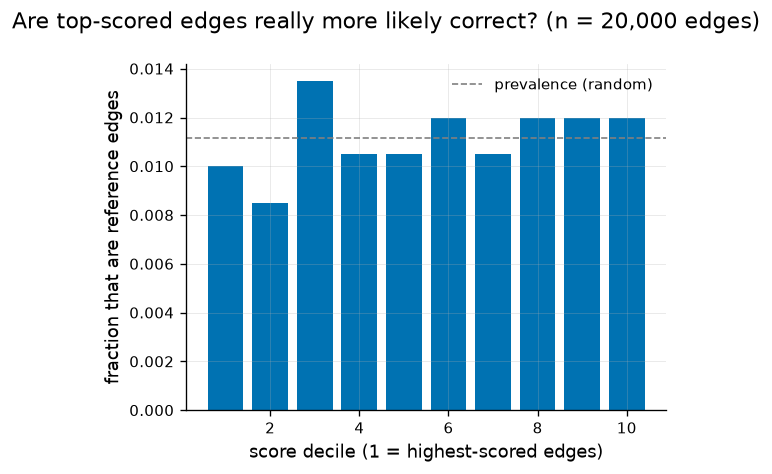
\includegraphics[width=0.85\linewidth]{../viz/calibration_cxg__10x-3-v2__homo-sapiens__breast__44941fdb.png}
\caption{-   (n = 20000 edges) - built from  grnboost2.tsv.gz}
\end{figure}
\begin{figure}[H]\centering
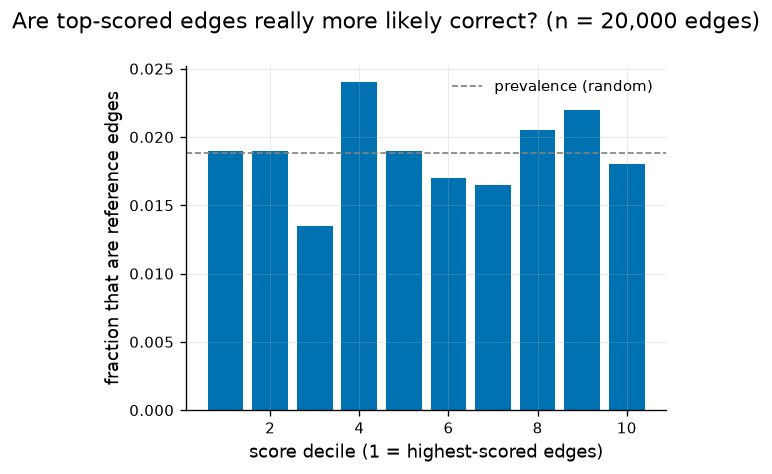
\includegraphics[width=0.85\linewidth]{../viz/calibration_cxg__10x-3-v2__homo-sapiens__cortex-of-kidney__2fc9c59f.png}
\caption{-   (n = 20000 edges) - built from  grnboost2.tsv.gz}
\end{figure}
\begin{figure}[H]\centering
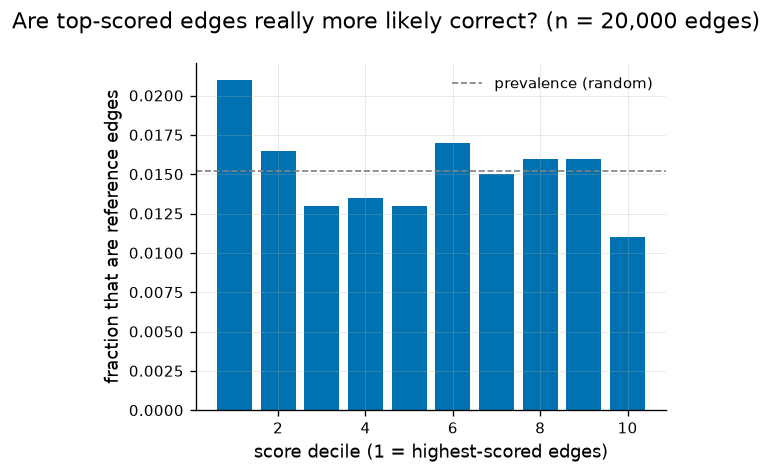
\includegraphics[width=0.85\linewidth]{../viz/calibration_cxg__10x-3-v2__homo-sapiens__duodenum__ee195b7d.png}
\caption{-   (n = 20000 edges) - built from  grnboost2.tsv.gz}
\end{figure}
\begin{figure}[H]\centering
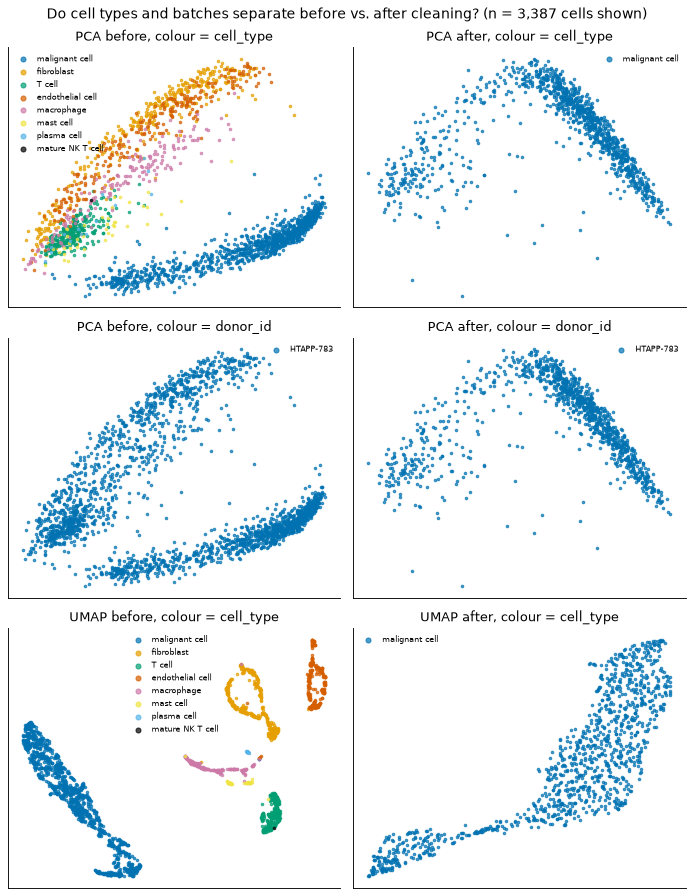
\includegraphics[width=0.85\linewidth]{../viz/embed_cxg__10x-3-v2__homo-sapiens__breast__44941fdb.png}
\caption{-   (n = 2276 cells) - built from  tasks.json (raw data)}
\end{figure}
\begin{figure}[H]\centering
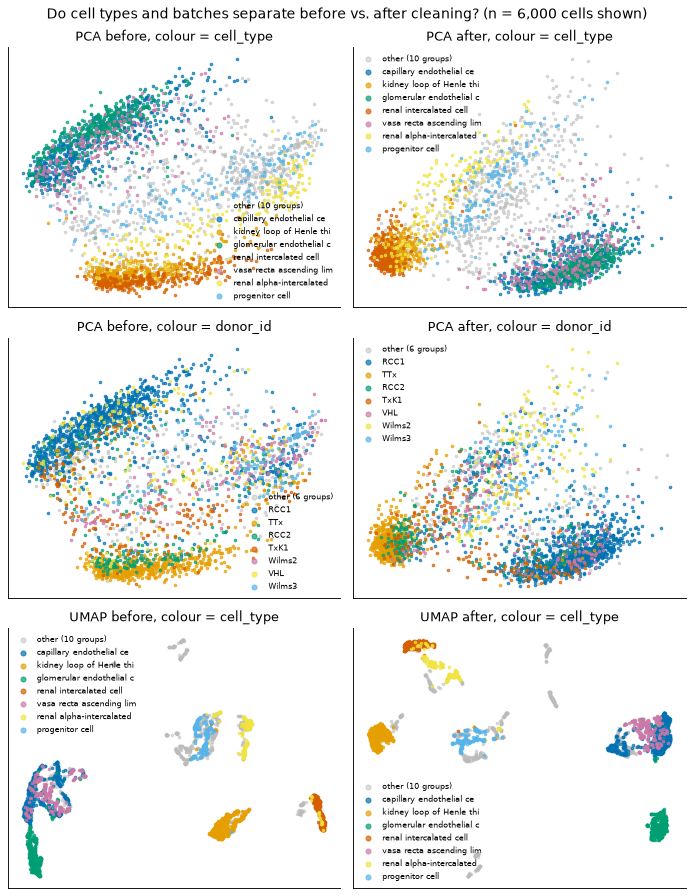
\includegraphics[width=0.85\linewidth]{../viz/embed_cxg__10x-3-v2__homo-sapiens__cortex-of-kidney__2fc9c59f.png}
\caption{-   (n = 4620 cells) - built from  tasks.json (raw data)}
\end{figure}
\begin{figure}[H]\centering
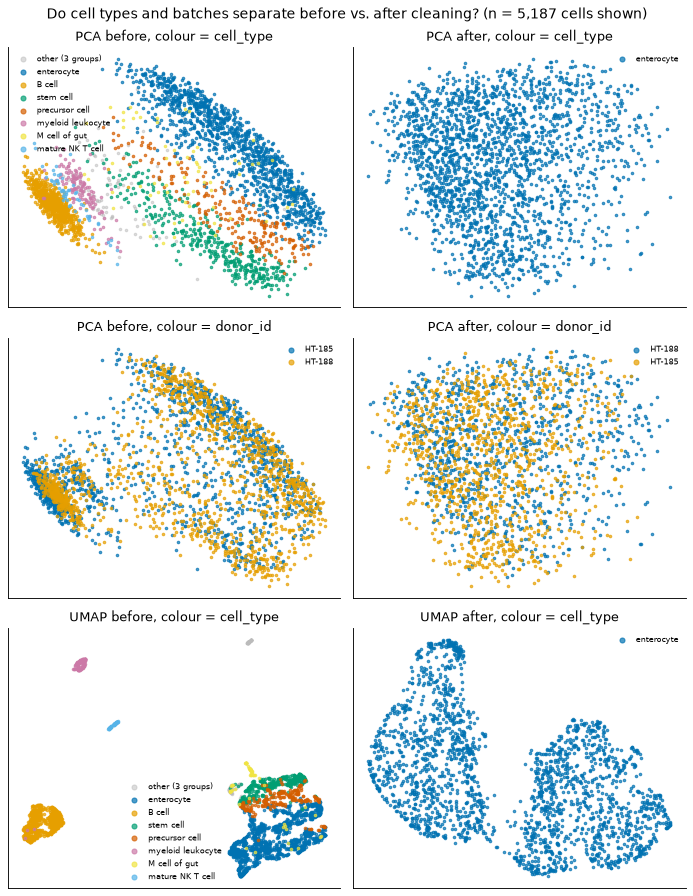
\includegraphics[width=0.85\linewidth]{../viz/embed_cxg__10x-3-v2__homo-sapiens__duodenum__ee195b7d.png}
\caption{-   (n = 5200 cells) - built from  tasks.json (raw data)}
\end{figure}
\begin{figure}[H]\centering
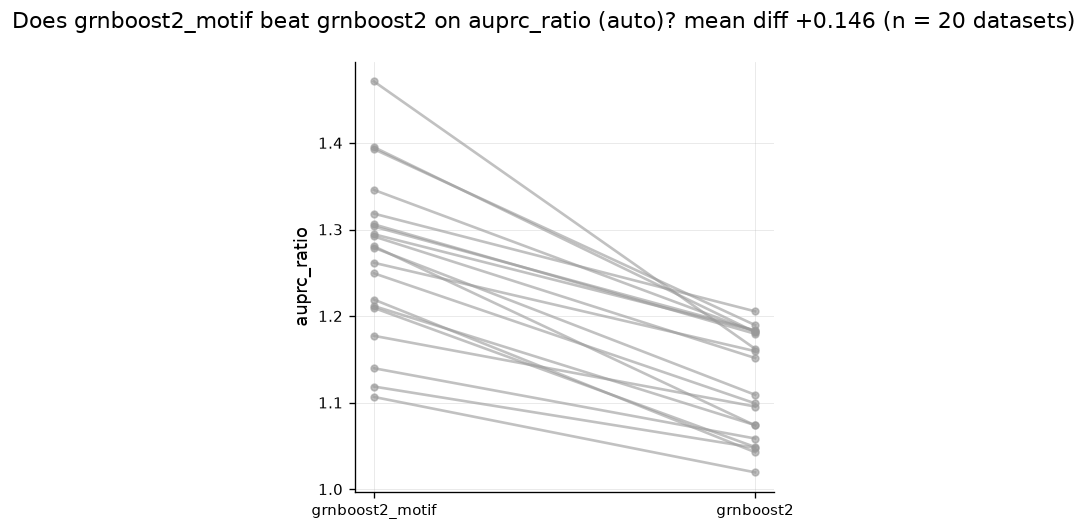
\includegraphics[width=0.85\linewidth]{../viz/lift_grnboost2_motif_vs_grnboost2.png}
\caption{-   (n = 20 datasets) - built from  rows/ .json (grnboost2\_motif vs grnboost2)}
\end{figure}
\begin{figure}[H]\centering
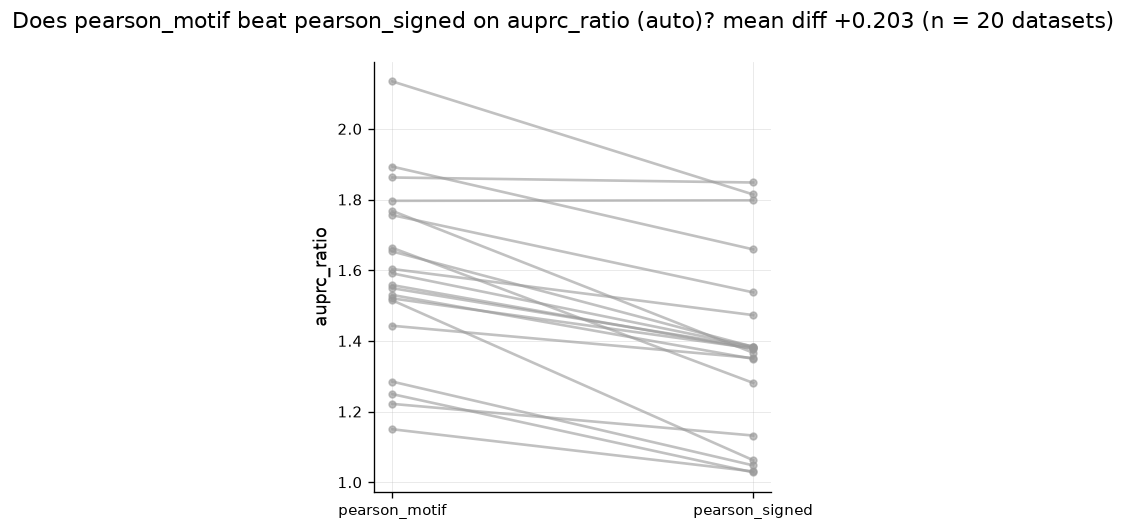
\includegraphics[width=0.85\linewidth]{../viz/lift_pearson_motif_vs_pearson_signed.png}
\caption{-   (n = 20 datasets) - built from  rows/ .json (pearson\_motif vs pearson\_signed)}
\end{figure}
\begin{figure}[H]\centering
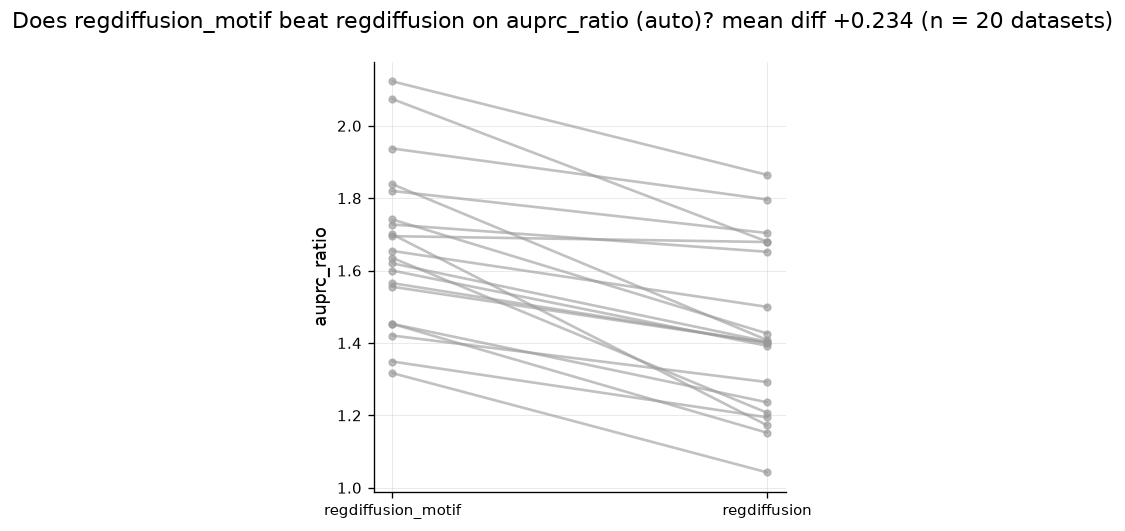
\includegraphics[width=0.85\linewidth]{../viz/lift_regdiffusion_motif_vs_regdiffusion.png}
\caption{-   (n = 20 datasets) - built from  rows/ .json (regdiffusion\_motif vs regdiffusion)}
\end{figure}
\begin{figure}[H]\centering
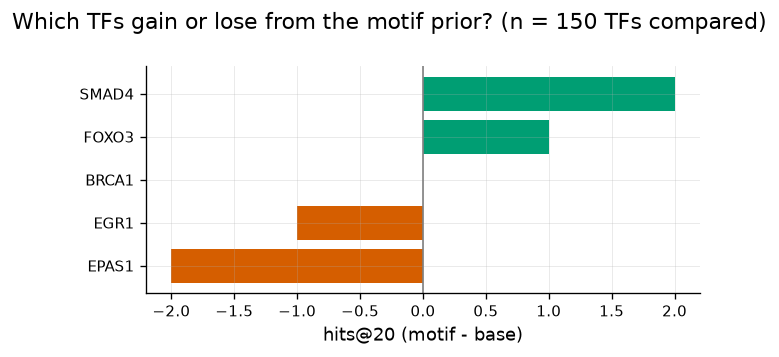
\includegraphics[width=0.85\linewidth]{../viz/motif_lift_cxg__10x-3-v2__homo-sapiens__breast__44941fdb_grnboost2.png}
\caption{-   (n = shared TFs) - built from  grnboost2.tsv.gz vs grnboost2\_motif.tsv.gz}
\end{figure}
\begin{figure}[H]\centering
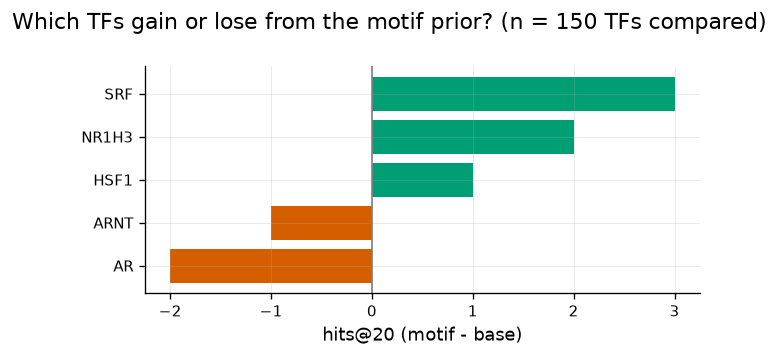
\includegraphics[width=0.85\linewidth]{../viz/motif_lift_cxg__10x-3-v2__homo-sapiens__breast__44941fdb_pearson_signed.png}
\caption{-   (n = shared TFs) - built from  pearson\_signed.tsv.gz vs pearson\_motif.tsv.gz}
\end{figure}
\begin{figure}[H]\centering
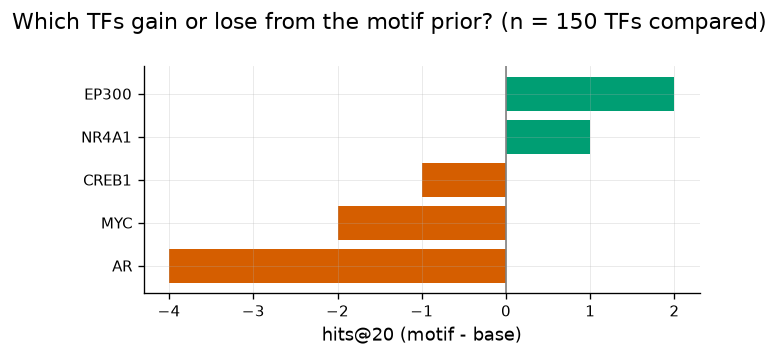
\includegraphics[width=0.85\linewidth]{../viz/motif_lift_cxg__10x-3-v2__homo-sapiens__breast__44941fdb_regdiffusion.png}
\caption{-   (n = shared TFs) - built from  regdiffusion.tsv.gz vs regdiffusion\_motif.tsv.gz}
\end{figure}
\begin{figure}[H]\centering
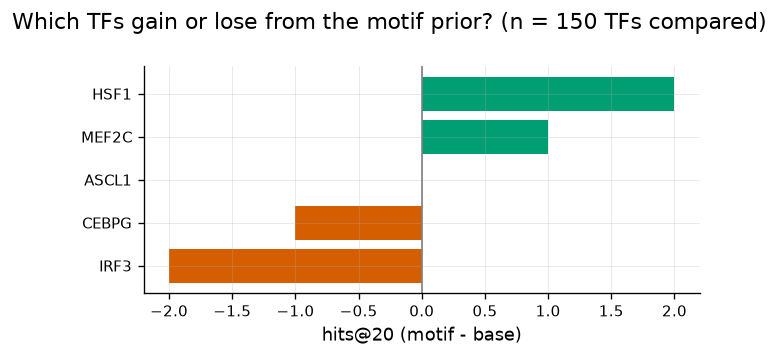
\includegraphics[width=0.85\linewidth]{../viz/motif_lift_cxg__10x-3-v2__homo-sapiens__cortex-of-kidney__2fc9c59f_grnboost2.png}
\caption{-   (n = shared TFs) - built from  grnboost2.tsv.gz vs grnboost2\_motif.tsv.gz}
\end{figure}
\begin{figure}[H]\centering
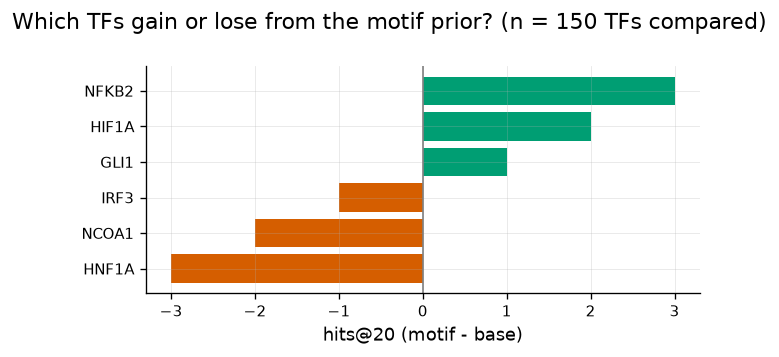
\includegraphics[width=0.85\linewidth]{../viz/motif_lift_cxg__10x-3-v2__homo-sapiens__cortex-of-kidney__2fc9c59f_pearson_signed.png}
\caption{-   (n = shared TFs) - built from  pearson\_signed.tsv.gz vs pearson\_motif.tsv.gz}
\end{figure}
\begin{figure}[H]\centering
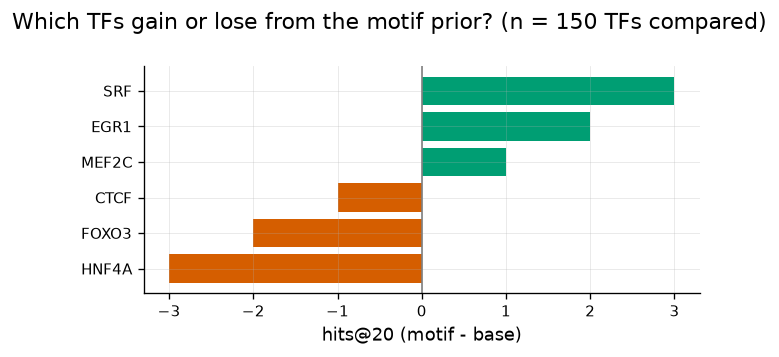
\includegraphics[width=0.85\linewidth]{../viz/motif_lift_cxg__10x-3-v2__homo-sapiens__cortex-of-kidney__2fc9c59f_regdiffusion.png}
\caption{-   (n = shared TFs) - built from  regdiffusion.tsv.gz vs regdiffusion\_motif.tsv.gz}
\end{figure}
\begin{figure}[H]\centering
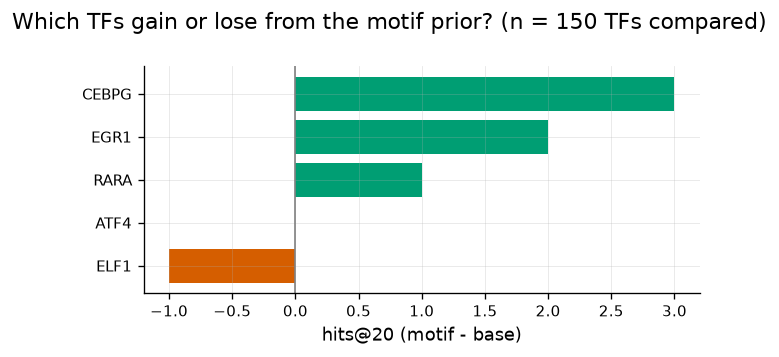
\includegraphics[width=0.85\linewidth]{../viz/motif_lift_cxg__10x-3-v2__homo-sapiens__duodenum__ee195b7d_grnboost2.png}
\caption{-   (n = shared TFs) - built from  grnboost2.tsv.gz vs grnboost2\_motif.tsv.gz}
\end{figure}
\begin{figure}[H]\centering
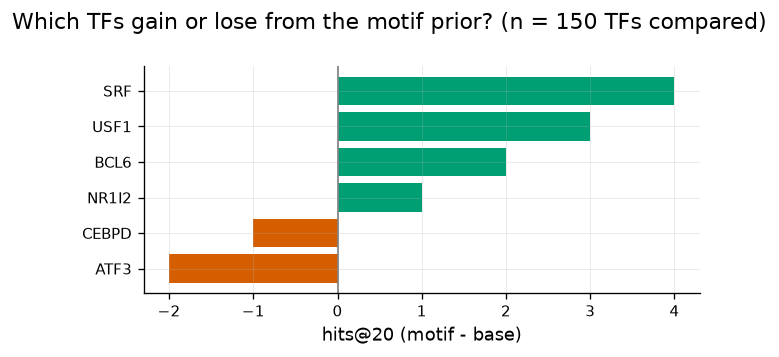
\includegraphics[width=0.85\linewidth]{../viz/motif_lift_cxg__10x-3-v2__homo-sapiens__duodenum__ee195b7d_pearson_signed.png}
\caption{-   (n = shared TFs) - built from  pearson\_signed.tsv.gz vs pearson\_motif.tsv.gz}
\end{figure}
\begin{figure}[H]\centering
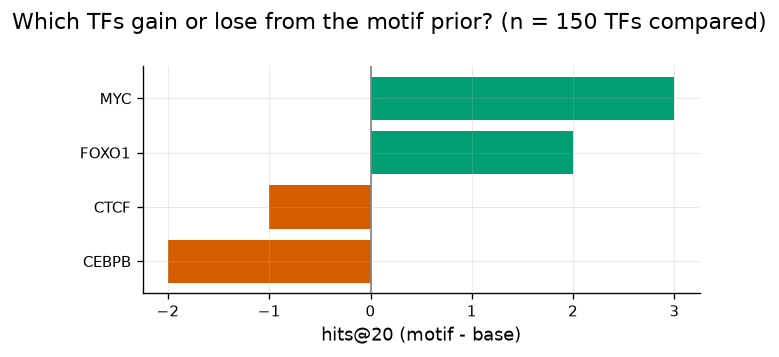
\includegraphics[width=0.85\linewidth]{../viz/motif_lift_cxg__10x-3-v2__homo-sapiens__duodenum__ee195b7d_regdiffusion.png}
\caption{-   (n = shared TFs) - built from  regdiffusion.tsv.gz vs regdiffusion\_motif.tsv.gz}
\end{figure}
\begin{figure}[H]\centering
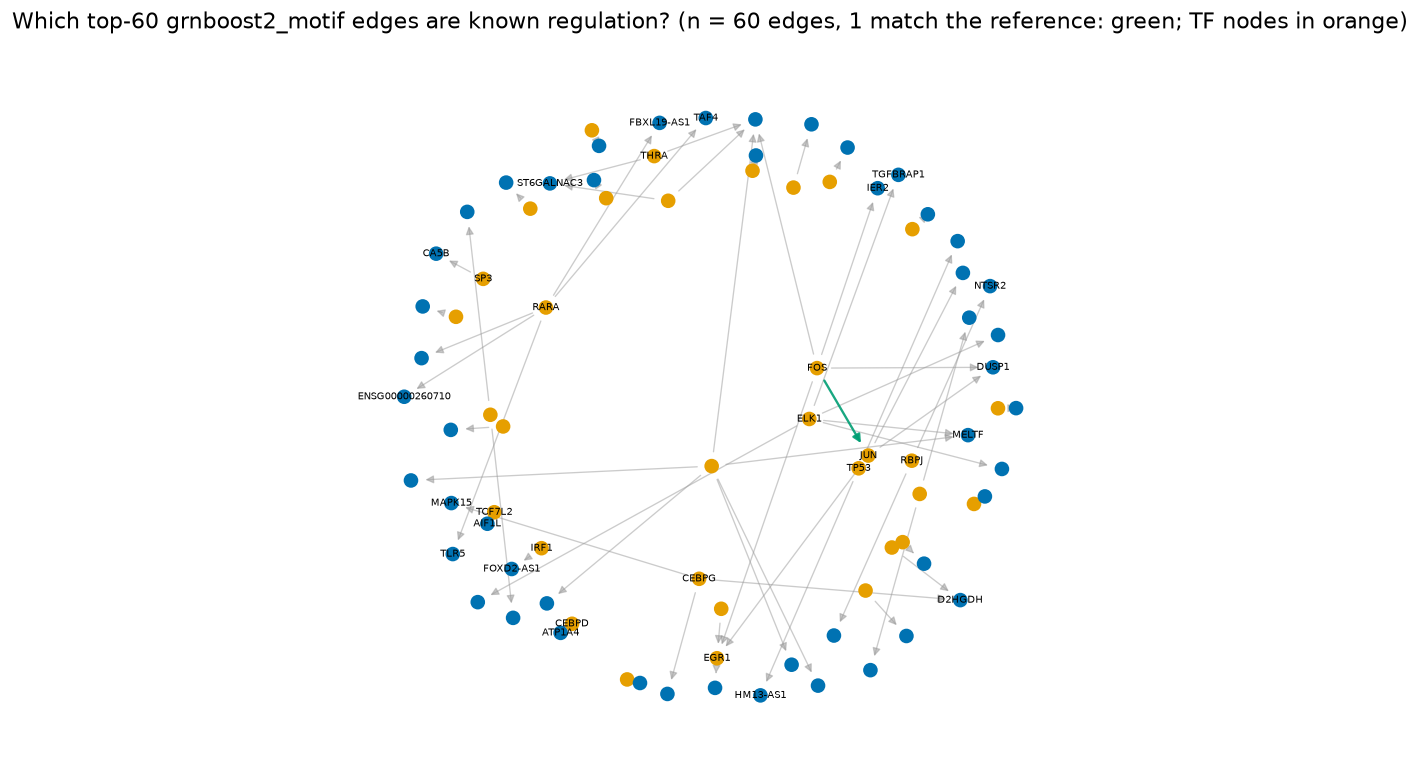
\includegraphics[width=0.85\linewidth]{../viz/network_cxg__10x-3-v2__homo-sapiens__breast__44941fdb.png}
\caption{-   (n = 60 edges) - built from  grnboost2\_motif.tsv.gz}
\end{figure}
\begin{figure}[H]\centering
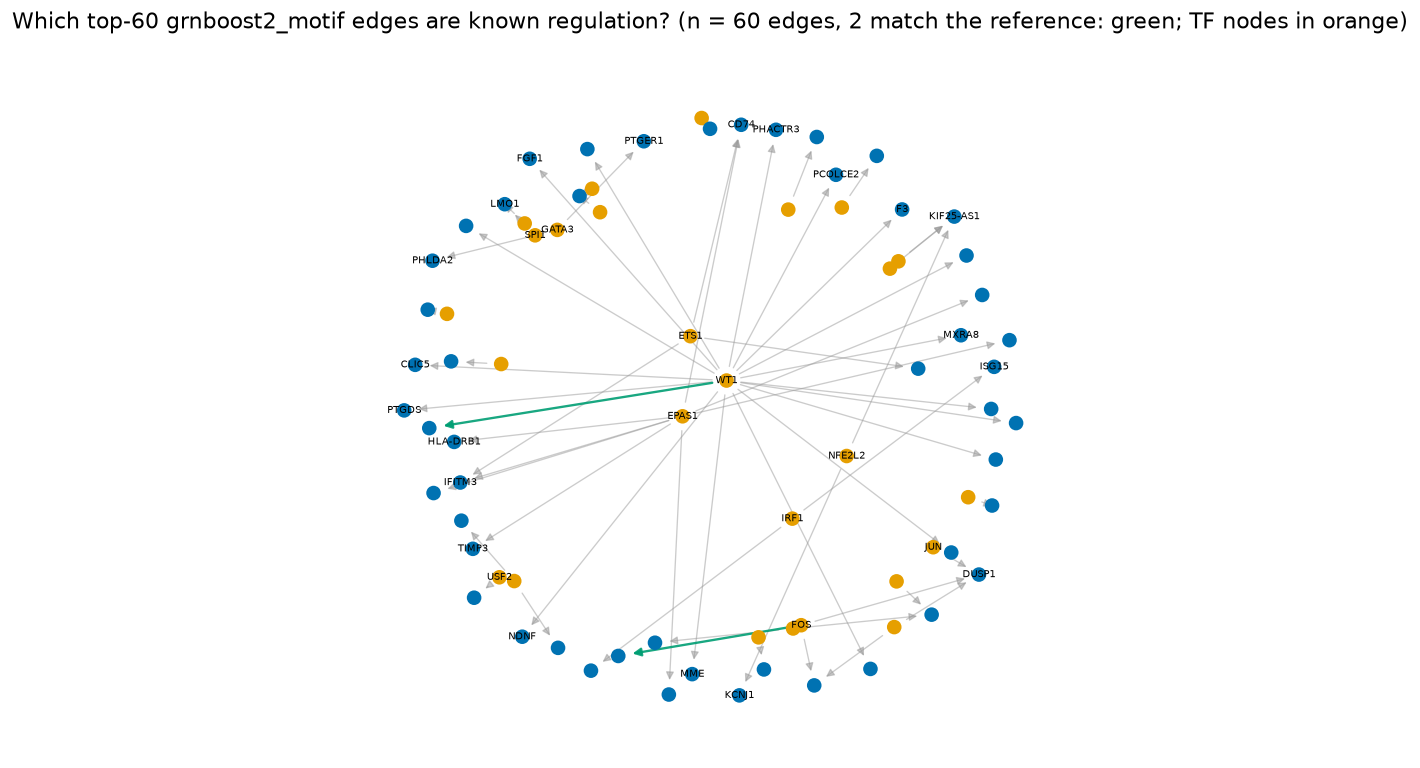
\includegraphics[width=0.85\linewidth]{../viz/network_cxg__10x-3-v2__homo-sapiens__cortex-of-kidney__2fc9c59f.png}
\caption{-   (n = 60 edges) - built from  grnboost2\_motif.tsv.gz}
\end{figure}
\begin{figure}[H]\centering
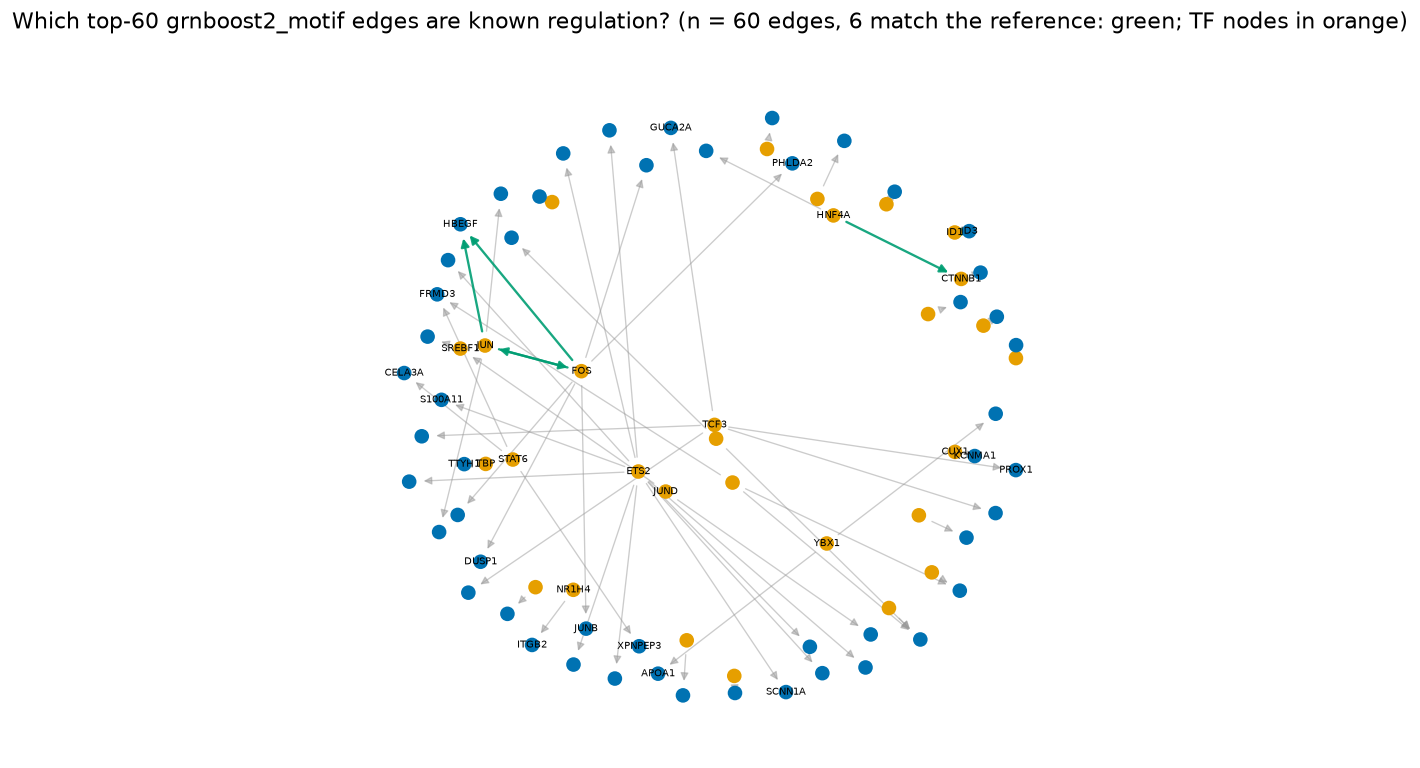
\includegraphics[width=0.85\linewidth]{../viz/network_cxg__10x-3-v2__homo-sapiens__duodenum__ee195b7d.png}
\caption{-   (n = 60 edges) - built from  grnboost2\_motif.tsv.gz}
\end{figure}
\begin{figure}[H]\centering
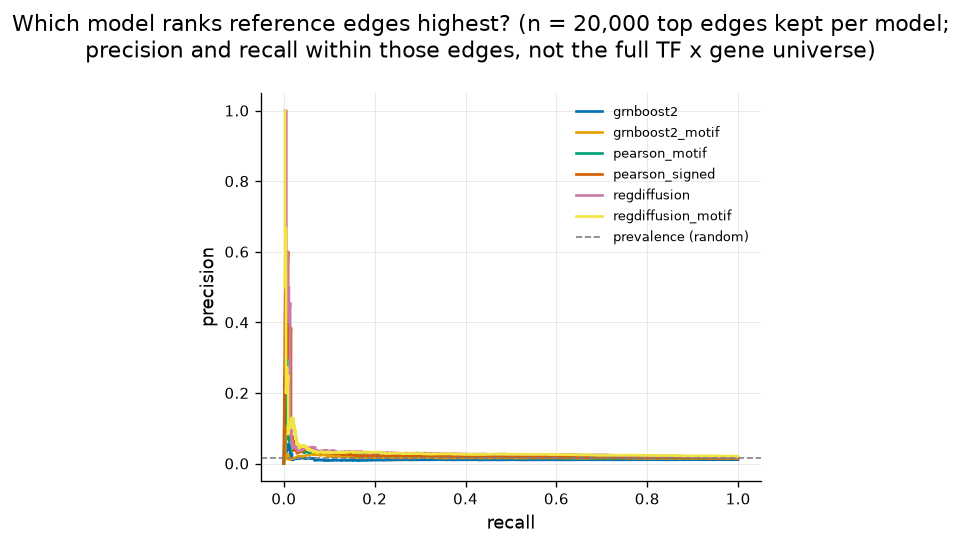
\includegraphics[width=0.85\linewidth]{../viz/pr_cxg__10x-3-v2__homo-sapiens__breast__44941fdb.png}
\caption{-   (n = 20000 edges) - built from  artifacts/cxg\_\_10x-3-v2\_\_homo-sapiens\_\_breast\_\_44941fdb/auto/ctx0}
\end{figure}
\begin{figure}[H]\centering
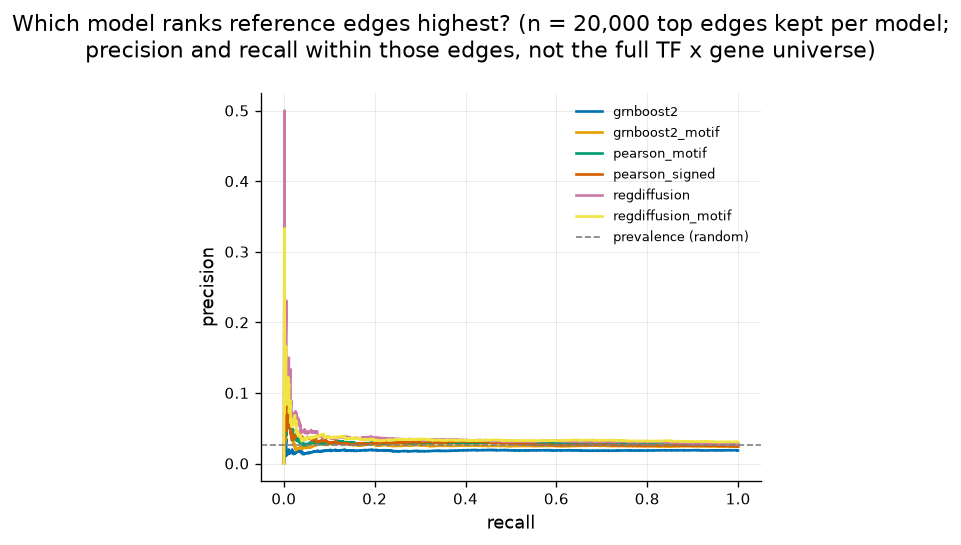
\includegraphics[width=0.85\linewidth]{../viz/pr_cxg__10x-3-v2__homo-sapiens__cortex-of-kidney__2fc9c59f.png}
\caption{-   (n = 20000 edges) - built from  artifacts/cxg\_\_10x-3-v2\_\_homo-sapiens\_\_cortex-of-kidney\_\_2fc9c59f/auto/ctx0}
\end{figure}
\begin{figure}[H]\centering
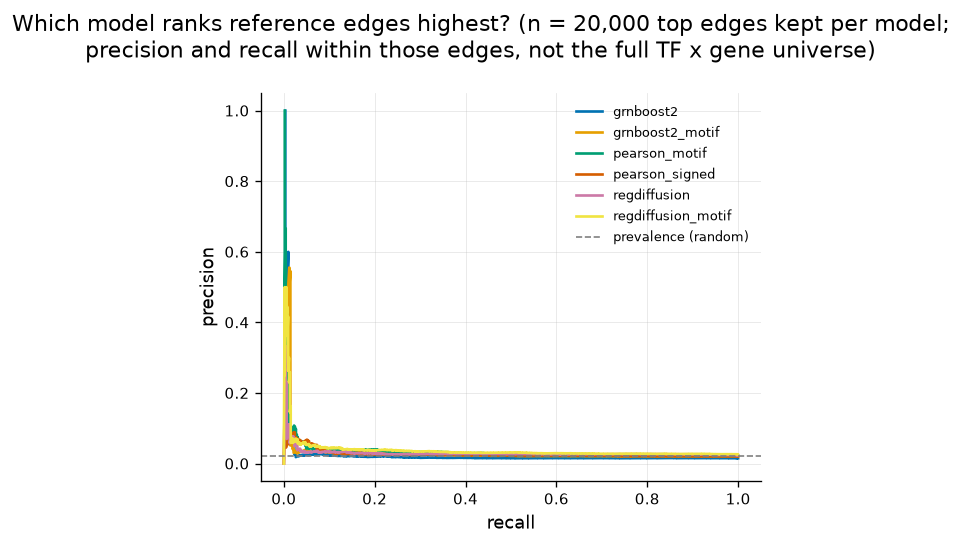
\includegraphics[width=0.85\linewidth]{../viz/pr_cxg__10x-3-v2__homo-sapiens__duodenum__ee195b7d.png}
\caption{-   (n = 20000 edges) - built from  artifacts/cxg\_\_10x-3-v2\_\_homo-sapiens\_\_duodenum\_\_ee195b7d/auto/ctx0}
\end{figure}
\begin{figure}[H]\centering
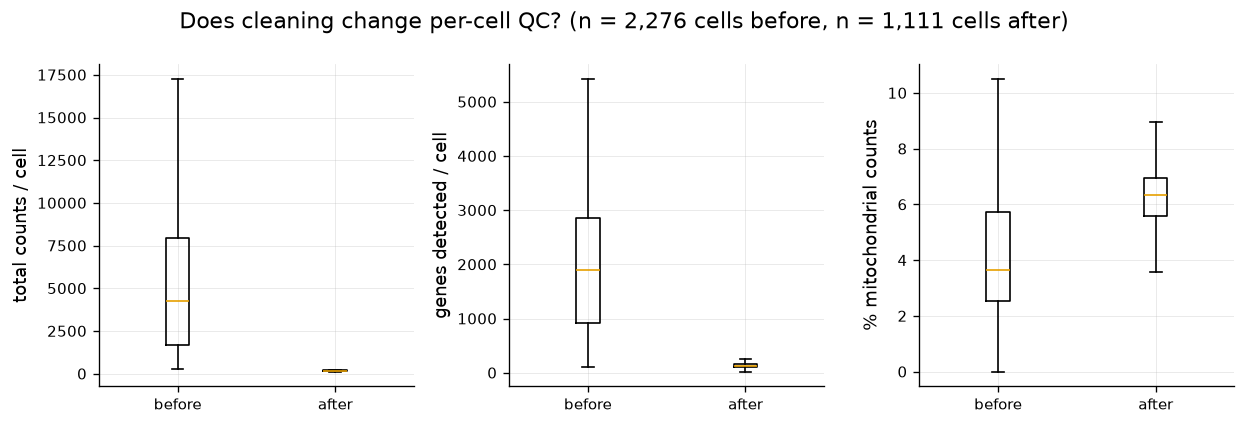
\includegraphics[width=0.85\linewidth]{../viz/qc_cxg__10x-3-v2__homo-sapiens__breast__44941fdb.png}
\caption{-   (n = 2276 cells) - built from  tasks.json (raw data)}
\end{figure}
\begin{figure}[H]\centering
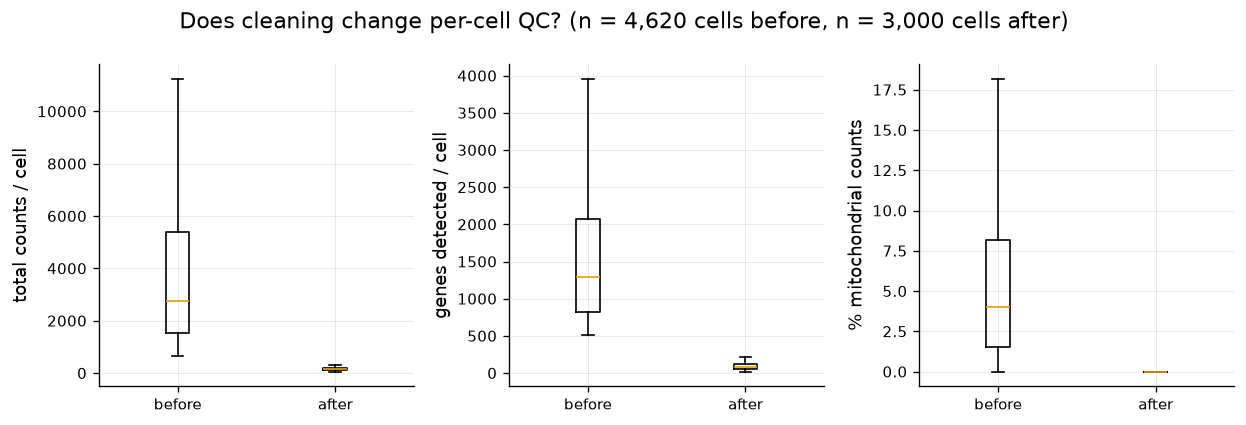
\includegraphics[width=0.85\linewidth]{../viz/qc_cxg__10x-3-v2__homo-sapiens__cortex-of-kidney__2fc9c59f.png}
\caption{-   (n = 4620 cells) - built from  tasks.json (raw data)}
\end{figure}
\begin{figure}[H]\centering
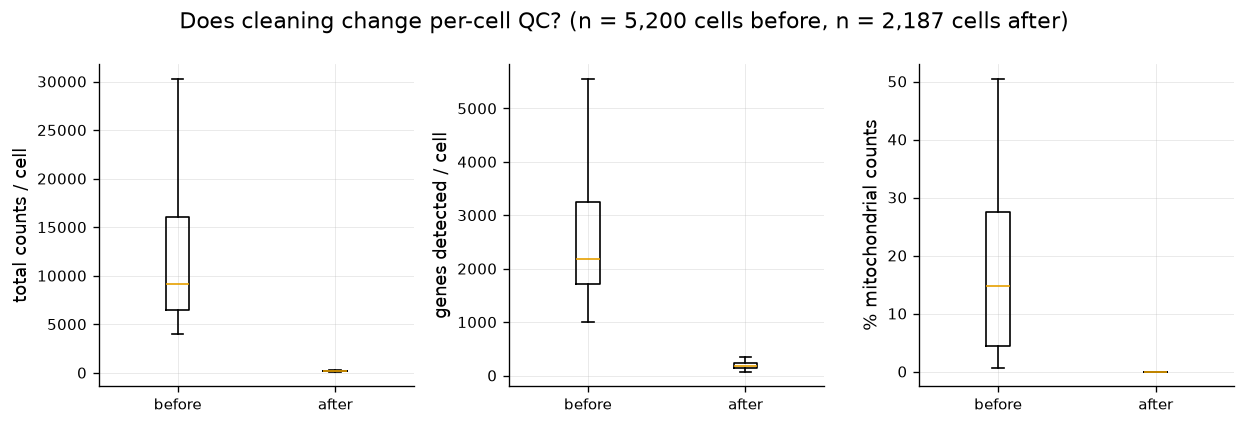
\includegraphics[width=0.85\linewidth]{../viz/qc_cxg__10x-3-v2__homo-sapiens__duodenum__ee195b7d.png}
\caption{-   (n = 5200 cells) - built from  tasks.json (raw data)}
\end{figure}
\begin{figure}[H]\centering
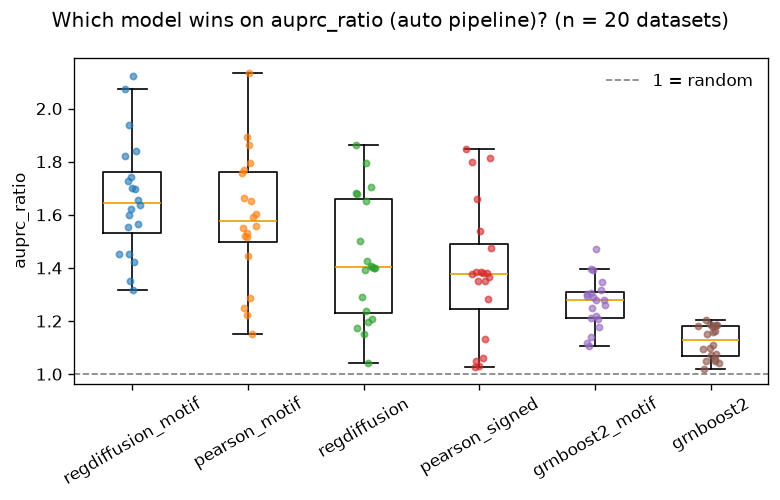
\includegraphics[width=0.85\linewidth]{../viz/scores_auprc_ratio_auto.png}
\caption{-   (n = 20 datasets) - built from  rows/ .json (auto/auprc\_ratio)}
\end{figure}
\begin{figure}[H]\centering
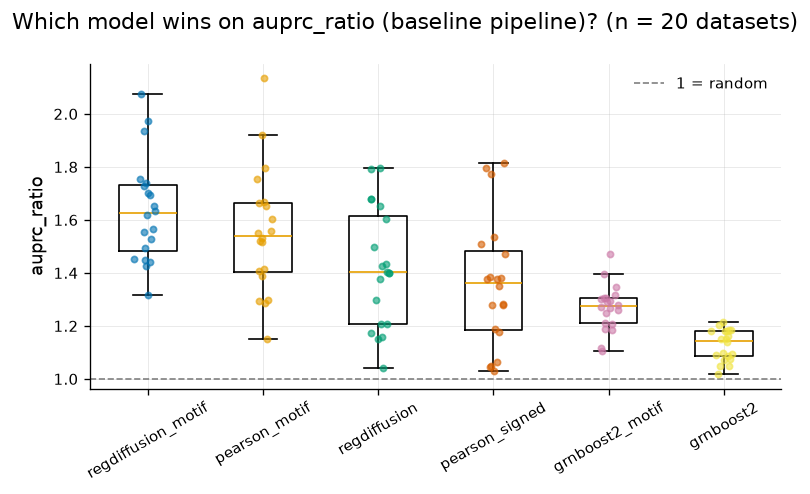
\includegraphics[width=0.85\linewidth]{../viz/scores_auprc_ratio_baseline.png}
\caption{-   (n = 20 datasets) - built from  rows/ .json (baseline/auprc\_ratio)}
\end{figure}
\begin{figure}[H]\centering
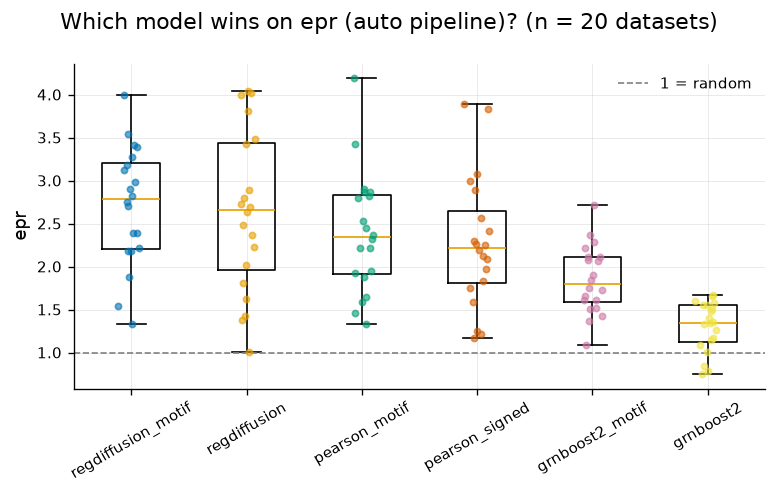
\includegraphics[width=0.85\linewidth]{../viz/scores_epr_auto.png}
\caption{-   (n = 20 datasets) - built from  rows/ .json (auto/epr)}
\end{figure}
\begin{figure}[H]\centering
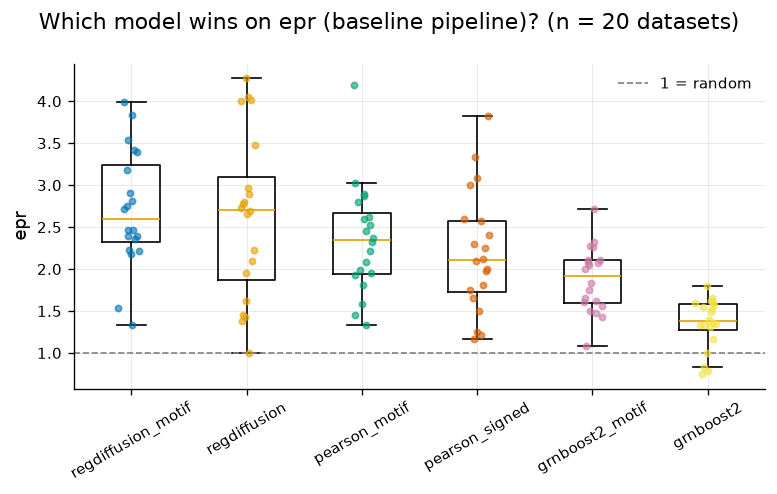
\includegraphics[width=0.85\linewidth]{../viz/scores_epr_baseline.png}
\caption{-   (n = 20 datasets) - built from  rows/ .json (baseline/epr)}
\end{figure}
\begin{figure}[H]\centering
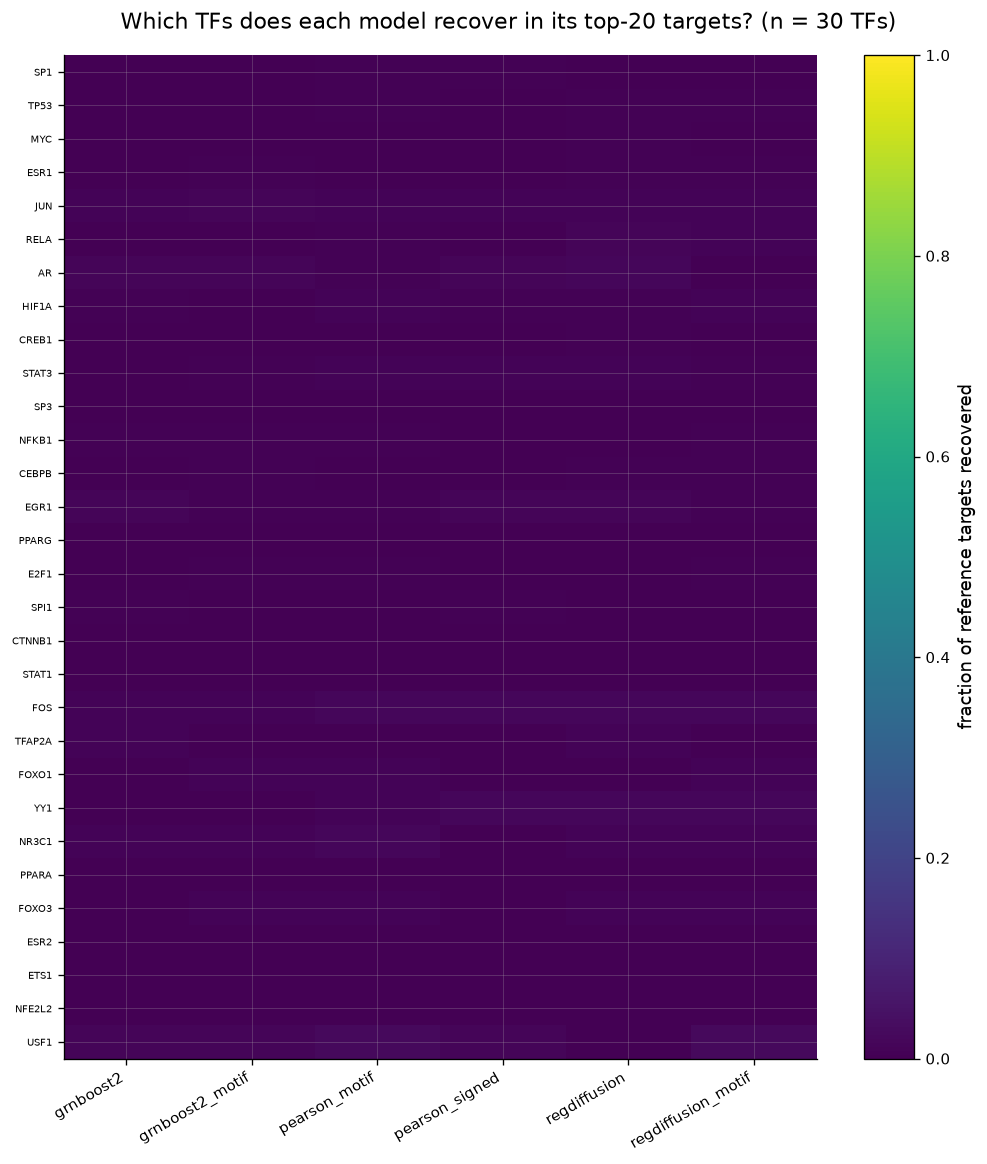
\includegraphics[width=0.85\linewidth]{../viz/tf_recovery_cxg__10x-3-v2__homo-sapiens__breast__44941fdb.png}
\caption{-   (n = up to 30 TFs) - built from  artifacts/cxg\_\_10x-3-v2\_\_homo-sapiens\_\_breast\_\_44941fdb/auto}
\end{figure}
\begin{figure}[H]\centering
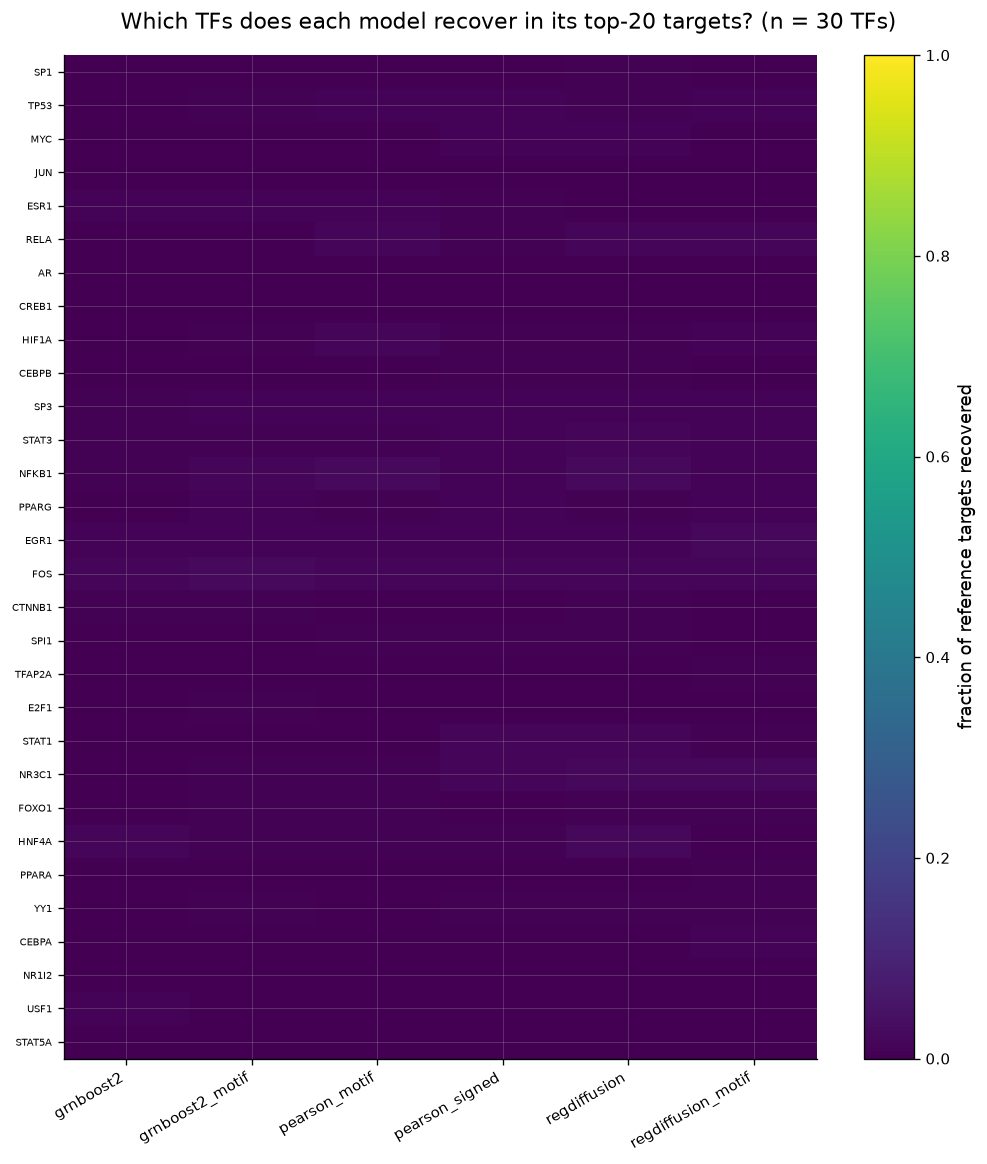
\includegraphics[width=0.85\linewidth]{../viz/tf_recovery_cxg__10x-3-v2__homo-sapiens__cortex-of-kidney__2fc9c59f.png}
\caption{-   (n = up to 30 TFs) - built from  artifacts/cxg\_\_10x-3-v2\_\_homo-sapiens\_\_cortex-of-kidney\_\_2fc9c59f/auto}
\end{figure}
\begin{figure}[H]\centering
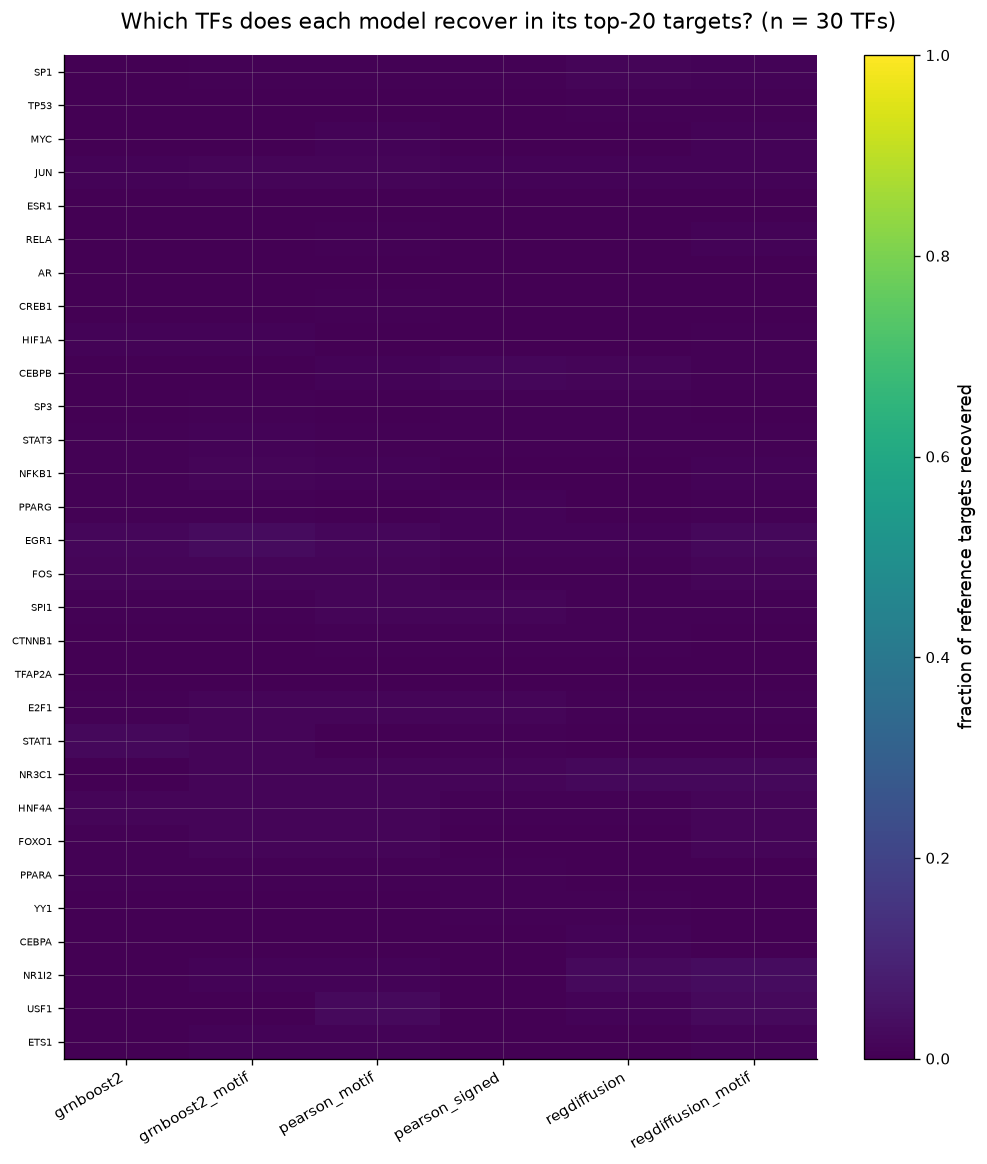
\includegraphics[width=0.85\linewidth]{../viz/tf_recovery_cxg__10x-3-v2__homo-sapiens__duodenum__ee195b7d.png}
\caption{-   (n = up to 30 TFs) - built from  artifacts/cxg\_\_10x-3-v2\_\_homo-sapiens\_\_duodenum\_\_ee195b7d/auto}
\end{figure}

\section{Limitations}
\begin{itemize}
\item None recorded.
\end{itemize}

\end{document}
